\documentclass[a4paper,12pt]{article}
% Define paper size, seperate titlepage, 12 pt. font, document class
%--------------------------------------------------------------------------------------------------
% Begin Preamble
%--------------------------------------------------------------------------------------------------
\usepackage{amsmath}
\usepackage{amssymb}
\usepackage{here}
\usepackage{graphicx}
\usepackage{epstopdf}
\usepackage{framed}
\usepackage{stmaryrd}
\usepackage{amsthm}
\usepackage{multicol}
\usepackage{manfnt}
\usepackage{fancybox}
\usepackage{pdflscape}
\usepackage{epsfig}
\usepackage{multirow}
\usepackage{color}
\usepackage{booktabs}
\usepackage{natbib}
\usepackage{lettrine}
\usepackage{appendix}
\usepackage{ifthen}
\usepackage[affil-it]{authblk}
\usepackage[utf8]{inputenc}
\usepackage[T1]{fontenc}
\usepackage{kpfonts}
\usepackage[doublespacing]{setspace}
\usepackage{csquotes}
\usepackage{subcaption}
%\usepackage{booktabs}
%\usepackage{threeparttable}
% Load Standard Packages
\usepackage{tabularx}
\newcolumntype{Y}{>{\centering\arraybackslash}X}
%Graphs and Tables to the end of the paper
\usepackage{endfloat}

%--------------------------------------------------------------------------------------------------
\usepackage{setspace}
	\onehalfspacing
% Set spacing to 1.5
%\numberwithin{figure}{section}
%\numberwithin{table}{section}
%  Number within Sections

\definecolor{deepred}{rgb}{0.803922,0,0}
%--------------------------------------------------------------------------------------------------
\usepackage{fancyhdr}
	\pagestyle{fancy}
	\headheight 35pt
	\fancyhf{}
	\rhead{}
	\chead{}
	\lhead{}
	\lhead{}
	\rfoot{\thepage}
	\cfoot{}
	\lfoot{}
	\renewcommand{\headrulewidth}{0.0pt}
	\renewcommand{\footrulewidth}{0.0pt}
% Define header and footnote styles
%--------------------------------------------------------------------------------------------------
%\usepackage[small,bf]{caption}
%\setlength{\captionmargin}{20pt}
% Makes the captions of figures/tables look nicely
%--------------------------------------------------------------------------------------------------
\usepackage[flushleft]{threeparttable}
\usepackage{ifxetex}
\usepackage[dvipsnames]{xcolor}
\ifxetex{%
  \usepackage{fontspec}
  \setmainfont{Linux Libertine O} % or any font on your system
  \newfontfamily\quotefont[Ligatures=TeX]{Linux Libertine O} % or any font on your system
\else
  \usepackage[utf8]{inputenc}
  \usepackage[T1]{fontenc}
  \usepackage{kpfonts} % or any other font package (or none)
  \newcommand*\quotefont{\fontfamily{fxl}} % selects Libertine for quote font
\fi
\usepackage{tikz}
\usepackage{framed}
% Make commands for the quotes
\newcommand*{\openquote}{\tikz[remember picture,overlay,xshift=-15pt,yshift=-10pt]
     \node (OQ) {\quotefont\fontsize{60}{60}\selectfont``};\kern0pt}
\newcommand*{\closequote}{\tikz[remember picture,overlay,xshift=15pt,yshift=10pt]
     \node (CQ) {\quotefont\fontsize{60}{60}\selectfont''};}
% select a colour for the shading
\definecolor{shadecolor}{named}{White}
% wrap everything in its own environment
\newenvironment{shadequote}%
{\begin{snugshade}\begin{quote}\openquote}
{\hfill\closequote\end{quote}\end{snugshade}}
%--------------------------------------------------------------------------------------------------
\usepackage[margin=2.3cm,includeheadfoot=false,twoside=false,bindingoffset=0.0cm,showframe=false]{geometry}
%\fancyhfoffset[E,O]{0pt}
% Add nicer enumbering of formulars
%--------------------------------------------------------------------------------------------------
\newcommand{\ws}{$^{\,\star}$}
\newcommand{\ms}{$^{\,\star \star}$}
\newcommand{\hs}{$^{\,\star \star \star}$}
\newcommand{\sym}[1]{\rlap{#1}}
% End Preamble
%--------------------------------------------------------------------------------------------------
\title{The political economy of EU asylum policies}
\date{September 2017}
\author[,1]{Martina Burmann\thanks{burmann@ifo.de}}
\author[,1]{Marcus Drometer\thanks{drometer@ifo.de}}
\author[,2]{Romuald M\'eango\thanks{meango@mea.mpisoc.mpg.de}}
\affil[1]{ifo Institute for Economic Research, Munich}
\affil[2]{Munich Center for the Economics of Aging (MEA)}
\renewcommand\Authands{ and }
%--------------------------------------------------------------------------------------------------
\begin{document}
%--------------------------------------------------------------------------------------------------
      \maketitle
%--------------------------------------------------------------------------------------------------

\begin{center}
PRELIMINARY - PLEASE DO NOT CITE WITHOUT PERMISSION
\end{center}
\begin{abstract}
\singlespacing
\noindent 
Asylum policies are partly determined by factors of political economy. However, there is little evidence on the precise linkages between political factors and asylum policies. We shed light on this issue by examining the impact of elections and parties on first-time asylum applications.  Our evidence is based on a large bilateral panel data set comprising 12 European destination countries and their 51 most relevant origin countries during the time period 2002 to 2014. Our findings suggest that  the number of asylum applicants under left- and right-wing parties converges before elections and differs thereafter. This result is robust to several different specifications and suggest that both left- and right-wing cabinets choose moderate policies before the election and less moderate policies after the election.
% * <burmann@ifo.de> 2017-09-04T14:21:33.467Z:
% 
% Decide whether to add the decision analysis and how to include that a different set of countries is used for the decision analysis.
% 
% ^ <burmann@ifo.de> 2017-09-07T15:50:57.948Z.
\bigskip

\textbf{Keywords}: Electoral cycles, migration policies.

\textbf{JEL}: H11, D72, F22

\bigskip
\end{abstract}
%\addtolength{\baselineskip}{.25\baselineskip}
\setcounter{page}{0} \renewcommand{\thepage}{}
\pagebreak\pagenumbering{arabic}\pagebreak

%%--------------------------------------------------------------------------------------------------
\section{Introduction}\label{Introduction}
Since March 2016, the European Union has signed an agreement with Turkey to close off the migration route across the Aegean, one of the most popular routes for asylum-seekers from Asia. This has been done despite protests from many human rights groups that think such an agreement violates the international Convention on Refugees. In a tribune entitled ``Keep them away'', \textit{\cite{Economist2017}} describes policies intended by many EU countries as policies ``where asylum-seekers would need to apply from abroad rather than coming to Europe.'' This tension between the provision of asylum for rightfully entitled individuals and groups, and the pursuit of other political and economic goals has been acknowledged by the economic literature that compares the provision of asylum as a public good, where costs are privately assumed by the host countries \citep{moraga2014}. With this background in mind, \cite{dustmann2016} note that ``the  different  exposures  to  refugee  inflows and  the  lack  of  any  effective  European-level  mechanism  to  `spread  the  burden'  of  hosting  refugee  populations,  led  many  countries  to  implement  procedures  aimed  at  reducing  inflows  into  their  territories.''

Despite the recognition that asylum policies are partly determined by political economy factors in the destination country, there is little empirical evidence on the precise linkages between those political factors and asylum policies. We shed light on this issue by examining the impact of elections and parties on first-time asylum applications.

Our evidence is based on a large bilateral panel data set from Eurostat reporting quarterly origin-specific first-time asylum applications for 12 European destination countries and their 51 most relevant origin countries during the time period 2002 to 2014. We combine this dataset with the ParlGov dataset that comprises information on European national elections (date and outcomes) and party positions \citep{parlgov2016}.

Our results establish empirically that asylum policies are affected by the electoral cycle and the identity of incumbent parties. More precisely, we establish two main results:
(i) before an election, the inflow of refugees is very similar across left and right cabinets; 
(ii)  in the quarters following an election, the inflow of refugees diverges substantially, with significantly less asylum applicants under a right-wing cabinet. These patterns are robust to several different specifications and suggest that both left- and right-wing cabinets choose moderate policies before the election and less moderate policies after the election.

Our paper is primarily linked to the literature that estimates the determinants of refugee inflows \citep{czaika2009, gudbrandsen2010, hatton2009, hatton2016, hatton2015,holzer2000, moore2007, neumayer2004, neumayer2005,toshkov2014}. We contribute to this literature by empirically demonstrating the importance of political factors in the destination countries. The main hypothesis of this paper is inspired by a well-established literature on the political budget cycle literature following \citet{nor75} which argues that incumbent politicians have strong incentives to distort public policies in order to increase approval rates whenever elections are pending.

In the upcoming version of the paper, we will also analyse the effect of elections and parties on decisions of asylum applications. Furthermore, we will use an IV-GMM procedure to address the potential problem that the outcome of an election might be influenced by short-term shocks that also affect the inflow of refugees. The remainder of the paper proceeds as follows: Section \ref{sec:data} introduces the data used for our analysis. Section \ref{sec:econometric} presents the econometric framework, and Section \ref{sec:results} describes the main results. Then, Section \ref{sec:robustness} discusses several robustness checks. Finally, Section \ref{sec:discussion} concludes with a discussion on the causality of the uncovered effects.

%[DISCUSS LITERATURE AND CONTRIBUTION]
 
\section{Data} \label{sec:data}

We use quarterly data on the number of  origin-specific first-time asylum applications  from a large bilateral panel data set from Eurostat. For our empirical analysis we select destination countries based on both data availability and size of the countries in terms of total first-time asylum applications in the time period 2002 to 2014. More precisely for our main specification we choose all countries which have data on origin-specific first-time asylum applications in at least 44 out of the 52 quarters under study and which report in total more than 30000 first-time asylum applications between 2002 and 2014.\footnote{If countries have missing information in 2008 or 2009 we impute this data from data on the origin-specific total applications in the respective quarters. This information is only available from 2008 onwards and, therefore, it is not possible to impute missing information for the years before 2008. For the exact calculation see the data section in the online appendix.}  We exclude Cyprus due to several irregular cabinet changes. The list of destination countries and the total number of first-time asylum applications in these countries is presented in Table 1.

\begin{table}[htbp]\centering
\caption{Total number of first-time asylum applications between 2002 and 2014 in 12 European destination countries}
\begin{tabular}{l r}
\hline \hline
\textbf{Destination country} & \textbf{\# of first-time  applications}  \\
\hline \hline
\smallskip
Germany &  704450 \\
\smallskip
France & 629288 \\
\smallskip
United Kingdom & 470960 \\
\smallskip
Sweden & 445525 \\
\smallskip
Belgium & 184200 \\
\smallskip
Netherlands & 167055 \\
\smallskip
Norway & 113545 \\
\smallskip 
Poland & 89680 \\
\smallskip
Denmark & 59440 \\
\smallskip
Spain & 56227 \\
\smallskip
Ireland & 47070 \\
\smallskip
Czech Republic & 35370 \\
\hline \hline
\multicolumn{2}{p{10cm}}{\footnotesize{Notes: The number of first-time applications represent the sum of  first-time applications in all available quarters from Quarter 1 2002 to Quarter 4 2014. For France the number of first-time applications in 2008 and for  Spain the number of first-time applications in 2008 and 2009 are imputed from the number of origin-specific applications in these years. For Belgium no data is available in 2004 and for Norway no data is available in 2002 and in Quarter 2, 3 and 4 of 2007.}}
\end{tabular}
\end{table}

We further select the top 51 origin countries which together account for more than 90\% of all first-time applications in the 12 destination countries between 2002 and 2014. As can be seen in Table 2 the top 10 origin countries already account for more than 45\% of the total first-time applications.\footnote{A full list of all 51 origin countries is provided in the online appendix. }


\begin{table}[htbp]\centering
\caption{Top 10 source countries and their share in the total first-time applications in the 12 destination countries from 2002 to 2014}
\begin{tabular}{l r r}
\hline \hline
\textbf{Source country} & \textbf{ Share of first-time  applications}   & \textbf{Cumulative share } \\
\hline \hline
\smallskip
Russia &  7.0\% & 7.0\% \\
\smallskip
Iraq & 6.9\%  & 13.9\% \\
\smallskip
Syria & 6.1\%  & 20.0 \%  \\
\smallskip
Afghanistan & 5.2 \% & 25.2\% \\
\smallskip
Somalia & 4.6\% & 29.8\%  \\
\smallskip
Iran & 3.4\% & 33.1\%  \\
\smallskip
Turkey  & 3.4\% & 36.5\% \\
\smallskip 
Eritrea & 3.3\% & 39.8\% \\
\smallskip
Serbia & 3.0\% & 42.9\% \\
\smallskip
Democratic Republic of Congo  & 2.8\% & 45.6\% \\
\hline \hline
\end{tabular}
\end{table}

Following \cite{hatton2016}, we drop country pairs with very few applications in order to avoid cases with zero applications in many quarters. We, thus, keep only country pairs with at least two first-time asylum applications per quarter on average, which leaves us with 480 out of 612 possible origin destination combinations.

We combine this dataset with the ParlGov dataset that comprises information on European national elections (date and outcomes) and party positions \citep{parlgov2016}. We derive the position of the government on a left-right scale by weighting the left-right position of the parties in government  against the ratio of the parties' seats to the cabinet's total seats in parliament. To illustrate that procedure here a simple numerical example: Assume the government of country X is formed by a coalition of two parties, A and B, with A having 60 and B having 80 seats out of the 200 total seats in parliament. Assume further that A scores 4 and B scores 5 on the left-right score, where 0 indicates extreme left and 10 indicates extreme right. The left-right position of the cabinet is, then, calculated as follows: 
\begin{equation*}
\tiny
LR~score~cabinet = LR~score~A * \frac{seats~A}{seats~A + seats~B} +LR~score~B * \frac{seats~B}{seats~A + seats~B} 
\end{equation*}which in the example would result in a left-right score of the cabinet of 4.57 ($4*\frac{60}{140} +5*\frac{80}{140})$.
After calculating this score for all cabinets of the 12 destination countries from 2002 to 2014, we next split the distribution of all cabinets in the sample at the median and code the cabinets below the median left and the cabinets above the median right. With the median cabinet left-right score in our baseline sample being 5.86, the cabinet in the above example would, thus, be coded as left.
Figure 1 illustrates the time-line of elections and cabinet changes in the destination countries.\footnote{Note that only cabinet changes where the cabinet group switches between left and right are marked in the graph. There are many more small cabinet changes which do not cause a change in the cabinet position group.}

\begin{figure}
	\centering
    	\caption{Cabinet changes and Elections in the destination countries 2002 to 2014}
	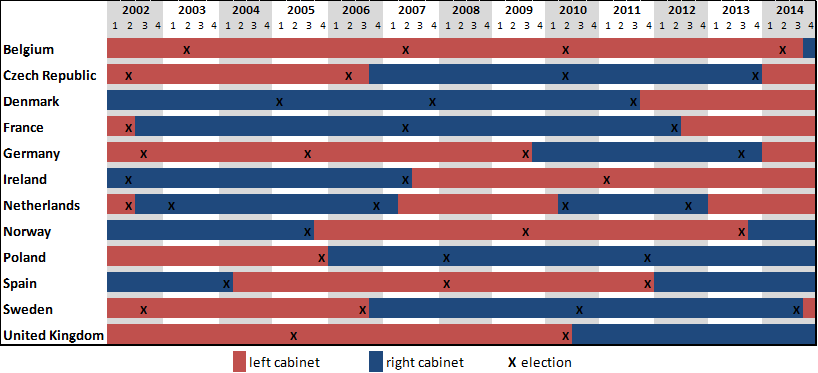
\includegraphics[width=1\textwidth]{elections_and_cabinet_changes.png}
	\label{Figure1}
\end{figure}

In order to account for the political and economic situation in the source countries we further add data on the Political Terror Scale \citep{PTS2016} , the Freedom House Index of Civic Liberties and Political Rights \citep{FHI2017}, the number of civil war battle death  as measured by the Uppsala Conflict Data Program \citep{Uppsala2017} and real GDP per capita from the Penn World Tables \citep{PWT2015}.  All of these variables except the number of civil war battle death vary only on the yearly level. As it seems plausible that  the decision to leave the origin country and to apply for asylum in another country is based on the situation in the origin country at the time leading up to the decision, we use the average values of origin specific variables from the current and the 3 previous quarters. The political terror scale in quarter 1 in 2005, for example, is consequently calculated as the mean of the political terror scale in 2005 and 3 times the political terror scale in 2004. 

To further capture the economic attractiveness of the destination countries we use data on the quarterly unemployment rates and the quarterly real GDP per capita in the destination countries from Eurostat. Finally, in some specifications we also include time-invariant bilateral information on the distance between origin and destination countries \citep{distance2017} and the number of adult immigrants from the origin country living in the destination country in 2000 \citep{Artucc2015}. Table 3 provides some descriptive statistics for the first-time asylum applications, the cabinet left-right score, as well as for the origin, destination and bilateral control variables.\footnote{More detailed information on the data sources, as well as on the definition and the calculation of the individual variables can be found in the data section in the online appendix.}

\begin{table}[htbp]\centering \caption{Summary statistics\label{sumstat}}
\begin{tabular}{p{8cm} c c c c c }\hline\hline
\multicolumn{1}{c}{Variable} & Obs & Mean & Std. Dev.
 & Min & Max  \\ \hline
Quarterly fist-time asylum applications & 23705 & 114.2 & 338.1 & 0 & 15330  \\
[0.5em]
Quarterly first-time asylum applications per 10000 inhabitants & 23705 & .1 & .2 & 0 & 11.3  \\
&\\
Cabinet left-right position  & 23705 & 5.6 & 1.5 & 2.8 & 8.2  \\
&\\
Political Terror Scale & 23705 & 3.3 & .9 & 1 & 5  \\
[0.5em]
Civic Liberty (FHI) & 23705 & 4.6 & 1.4 & 2 & 7  \\
[0.5em]
Political Rights (FHI) & 23705 & 4.9 & 1.7 & 1 & 7  \\
[0.5em]
Quarterly civil war battle death (000s) & 23705 & .3 & 1.3 & 0 & 17.6  \\
[0.5em]
Yearly real GDP per capita at origin & 23705 & 6440.8 & 5270.3 & 336.8 & 24039.1  \\

&\\
Distance from origin to destination & 23705 & 4395.2 & 2167.8 & 454 & 9680  \\
[0.5em]
Migrant stock in 2000/1 & 23705 & 16452.5 & 74737.4 & 0 & 1272000  \\

&\\
Quarterly real GDP per capita at destination & 23705 & 8717.2 & 3203.3 & 1557.5 & 18025.9  \\
[0.5em]
Quarterly unemployment rate at destination & 23705 & 7.8\% & 3.9\% & 2.4\% & 26.9\%  \\
\hline \hline
\end{tabular}
\end{table}

\section{Econometric specification} \label{sec:econometric}
In our main specification we estimate the following fixed-effect regression:
\begin{equation}
Y_{ijq} =\alpha_1 \mathbf{O_{iq}} + \alpha_2 \mathbf{D_{jq}} + \alpha_3 [\mathbf{Q_{j.}} *  \mathbf{C_{jq}}] + \tau_q + \sigma_{ij} +  \varepsilon_{ijt},
\end{equation}where the dependent variable ($Y_{ijq}$) represents the log of the number of first-time asylum applications per capita from citizens of origin country i in destination country j in quarter q. To derive this equation, we closely follow the specification of \cite{hatton2016}, and add to the origin and destination specific explanatory variables $\mathbf{O_{iq}}$ and $\mathbf{D_{jq}}$, a set of interaction terms of the ruling cabinet's position indicator $\mathbf{C_{jq}}$
 and  a set of dummies for before and and after the election ($\mathbf{Q_j.} := Q_{j,bef},  Q_{j,aft}$) or for different quarters before and after an election in a quarter $t=0$, in destination country $j$ ($\mathbf{Q_j.} =\{Q_{jt}, t = -6, \ldots, +6\}$).
 
  Similar to \cite{hatton2016}, we include Political Terror Scale, Freedom House Index of Civic Liberties, Freedom House Index of  Political Rights, number of battle deaths and log real GDP per capita in the vector of time variant origin specific variables $\mathbf{O_{iq}}$. The vector of time variant destination variables $\mathbf{D_{jq}}$ comprises of the quarterly log real GDP per capita and the quarterly unemployment rate at destination. 
  
 Our main specification as described in equation (1), moreover, includes quarter-year dummies $\tau_q$ and destination-origin fixed effects $\sigma_{ij}$. In all regressions standard errors are clustered by origin country.
 
 In the upcoming version of the paper, we further plan to look at three different asylum decision outcomes: (1) the overall acceptance rate defined as the ratio of all positive decisions to all decisions taken in that quarter, (2) the refugee status rate defined as the ratio of people who were granted full Geneva Convention refugee status to all people seeking refugee status and (3) the temporary protection rate defined as the ratio of other positive decisions to all decisions.  In order to control for the possible impact of the inflow of asylum seekers on the outcomes of asylum decisions, we additionally include  the log of the yearly total asylum decisions in the destination country as well as the log of  the yearly dyadic asylum decisions in the destination country in our regression equation (1) . 

\section{Results} \label{sec:results}
  Column (2) in Table \ref{tab:main_results} presents the results of the estimation of equation (1) for the outcome ``log first-time asylum applications per capita'' for the model with only two periods: before the election comprising of the 5 quarters before the election and the election quarter, and after the election comprising of the 6 quarters after the election.\footnote{Column (1) and (3) report results from similar regressions with different fixed effects.}  
  
 In line with the literature and the results of \citet{hatton2016}, we find that measures of political oppression and violence in the host country are positively correlated with the number of asylum applications. Moreover, the negative significant coefficient of the log origin country real GDP per capita suggests that also adverse economic conditions in the host countries drive asylum applications. As bad economic conditions are, however, often a byproduct of wars and political instability, this does not mean that asylum seekers leave their home country primarily for economic reasons. We moreover find a small negative effect of the unemployment rate in the destination country, which could indicate both, that a higher unemployment rate reduces the attractiveness of a destination country or that in times of higher unemployment more restrictive asylum policies are implemented. Interestingly, in contrast to \citet{hatton2016}, our results also indicate that a higher GDP per capita in the destination country is associated with fewer asylum applications. 
% * <burmann@ifo.de> 2017-09-07T12:40:45.398Z:
% 
% Possible Explanation/Interpretation of that? Do you have any ideas why that could make sense? Richer countries are more effective in keeping refugees away? 
% 
% ^.
 \begin{table}[htbp]\centering
\def\sym#1{\ifmmode^{#1}\else\(^{#1}\)\fi}
\caption{Determinants of log(First time asylum applications per capita)}
\begin{tabular}{l*{3}{c}}
\hline\hline
                    &\multicolumn{1}{c}{(1)}         &\multicolumn{1}{c}{(2)}         &\multicolumn{1}{c}{(3)}         \\
\hline
Political Terror Scale&       0.408\sym{***}&       0.409\sym{***}&                     \\
                    &    (0.0709)         &    (0.0702)         &                     \\
[0.5em]
Civic Liberty (FHI) &       0.181         &       0.182         &                     \\
                    &     (0.130)         &     (0.128)         &                     \\
[0.5em]
Political Rights (FHI)&      0.0411         &      0.0423         &                     \\
                    &    (0.0758)         &    (0.0757)         &                     \\
[0.5em]
Quarterly civil war battle death (000s)&       0.138\sym{***}&       0.137\sym{***}&                     \\
                    &    (0.0154)         &    (0.0152)         &                     \\
[0.5em]
Log origin country real GDP per capita&      -0.644\sym{***}&      -0.646\sym{***}&                     \\
                    &     (0.173)         &     (0.170)         &                     \\
[0.5em]
Log migrant stock in 2000/1&       0.263\sym{***}&                     &       0.263\sym{***}\\
                    &    (0.0210)         &                     &    (0.0210)         \\
[0.5em]
Log distance from origin to destination&      -0.608\sym{*}  &                     &      -0.613\sym{*}  \\
                    &     (0.298)         &                     &     (0.296)         \\
[0.5em]
Log destination country real GDP per capita&      -1.440\sym{**} &      -1.515\sym{**} &      -1.185\sym{*}  \\
                    &     (0.492)         &     (0.441)         &     (0.467)         \\
[0.5em]
Quarterly unemployment rate at destination&     -0.0734\sym{***}&     -0.0746\sym{***}&     -0.0717\sym{***}\\
                    &    (0.0115)         &    (0.0108)         &    (0.0117)         \\
[0.5em]
Cabinet position left * Before the election&      0.0246         &      0.0231         &      0.0116         \\
                    &    (0.0291)         &    (0.0292)         &    (0.0304)         \\
[0.5em]
Cabinet position left * After the election&       0.122\sym{***}&       0.114\sym{***}&       0.116\sym{***}\\
                    &    (0.0238)         &    (0.0223)         &    (0.0240)         \\
[0.5em]
Cabinet position right * Before the election&      0.0361         &      0.0387         &      0.0371         \\
                    &    (0.0239)         &    (0.0227)         &    (0.0238)         \\
[0.5em]
Cabinet position right * After the election&     -0.0930\sym{***}&     -0.0874\sym{***}&     -0.0950\sym{***}\\
                    &    (0.0244)         &    (0.0234)         &    (0.0241)         \\
\hline
Observations        &       23705         &       23705         &       23705         \\
Adjusted \(R^{2}\)  &       0.444         &       0.177         &       0.447         \\
Fixed Effects       &           O         &       D x O         &       O x T         \\
Destination dummies &         Yes         &          No         &         Yes         \\
Quarter-Year dummies&         Yes         &         Yes         &          No         \\
\hline\hline
\multicolumn{4}{l}{\footnotesize Standard errors in parentheses: \sym{*} \(p<0.05\), \sym{**} \(p<0.01\), \sym{***} \(p<0.001\)}\\
\end{tabular}
\label{tab:main_results}
\end{table}
 
 Most importantly, our results, moreover, establish empirically that asylum policies are affected by the electoral cycle and the identity of incumbent parties. As illustrated in Figure \ref{main_results_bef-after} we find that in the time before an election the inflow of refugees is very similar across all types of cabinets, whereas in the quarters just after an election, the inflow of refugees diverges substantially, with significantly less asylum applicants under right-wing cabinets and significantly more asylum applicants under left-wing cabinets. 
 
 \begin{figure}
	\centering
    	\caption{Log First-Time Asylum Applications per Capita: Predicted pattern before and after an election}
	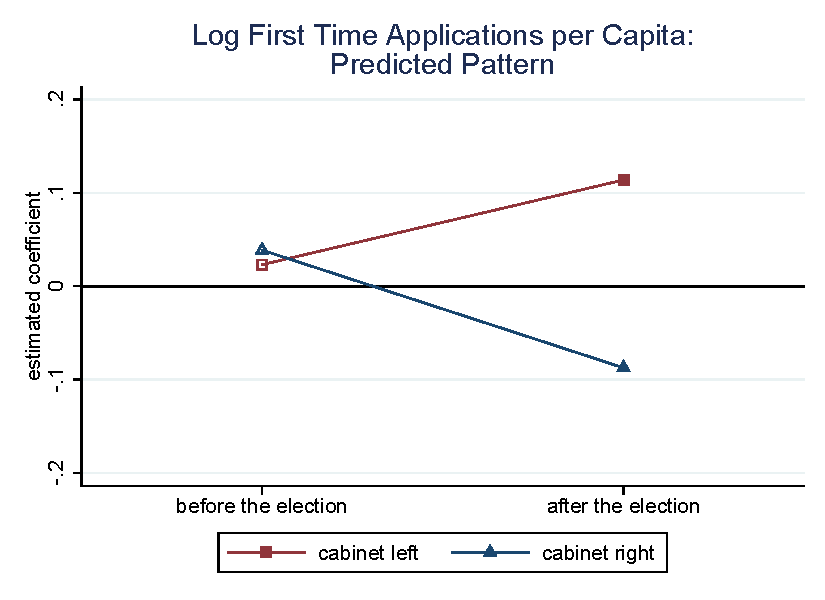
\includegraphics[width=1\textwidth]{app_Graph1.pdf}
    {\footnotesize This figure shows the time evolution of refugee inflows as estimated in the fixed effects regression (1) with a set of dummies for before and after the election. Significant coefficients are indicated by filled plot markers. }
	\label{main_results_bef-after}
\end{figure}

 Reassuringly, the results of the estimation with individual dummies for different quarters before and after an election, which are illustrated in Figure \ref{main_results_quarters}, confirm that the turning point is really the quarter following the election.  As highlighted in the next section this interesting pattern is robust to several different specifications and suggest that both left and right-wing cabinets choose moderate policies before the election and less moderate policies after the election.



\begin{figure}
	\centering
    \caption{Log First-Time Asylum Applications per Capita: Predicted pattern 6 quarters before and after an election}
	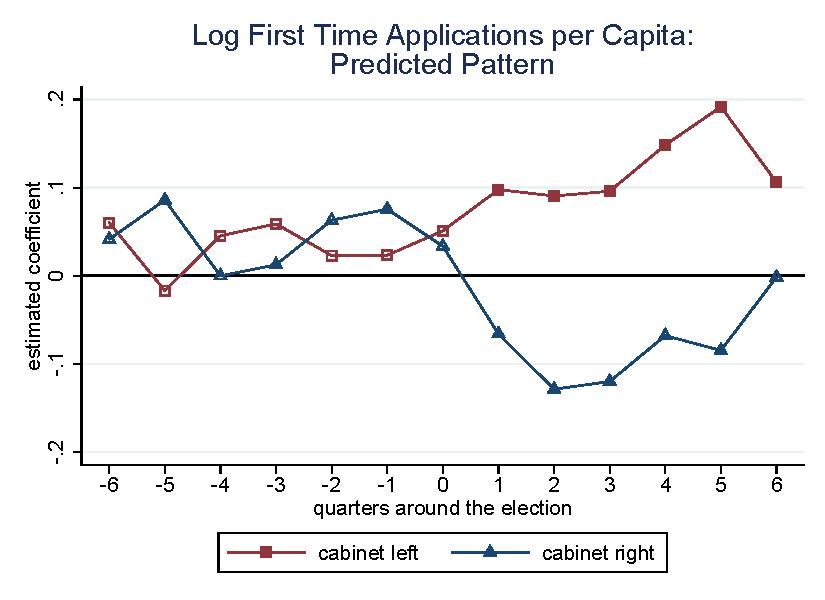
\includegraphics[width=1\textwidth]{app_Graph2.pdf}
	      {\footnotesize This figure shows the time evolution of refugee inflows as estimated in the fixed effects regression (1) with a set of dummies for different quarters before and after an election in a quarter $t=0$. Significant coefficients are indicated by filled plot markers. }\\
\label{main_results_quarters}
\end{figure}

\section{Robustness Checks}\label{sec:robustness}
Our first important robustness check confirms that our results are not sensitive to the choice of fixed effects. As can be seen in Table \ref{tab:main_results}, all coefficients are very similar to our main specification (column 2), if we instead of destination-origin fixed effects and time dummies, include origin fixed effects and destination and year dummies (column 1)  or origin-time fixed effects and destination dummies (column 3).  In the online appendix we further show that our main results hold if we control for the average asylum applications per capita in the previous 5 years, which indicates that election outcomes are not influenced by previous refugee inflows.  In order to account for the fact that in general refugee inflows might be different under right and left cabinets we conduct a further robustness check where we include a dummy for the incumbent's cabinet position  in addition to the interaction terms.  As the coefficient is very small and insignificant and the main results don't change we decide to drop the dummy for the incumbent's cabinet position in the main specification.  

A further concern is that some of our effects might be driven by the change in the data collection method by Eurostat in 2008. In order to account for that, we therefore also conduct a robustness check including a dummy which is equal to 1 if the year is 2008 or later and equal to zero if the year is 2002 to 2007. As the coefficient of this dummy is small and insignificant and the results don't change, we are confident that change in the collection method does not influence our results.  Several other robustness checks, moreover,  show that our results are not sensible to
\begin{itemize}
\itemsep0em 
\item  using the log of the number of first-time asylum applications per capita in the in the \textbf{origin} country as our dependent variable 
\item using  the current values of the origin country control variables instead of averages of the current and the past three quarters 
\item clustering the standard errors on the destination-origin level
\item normalizing the cabinet position on the country level before computing the cabinet position dummies (left and right)
\item leaving missing data on quarterly  first-time asylum applications for 2008 and 2009 missing instead of imputing it from the total applications
\item choosing  different cutoffs  for dropping countries pairs with few applications (one and three average applications per quarter)
\item looking only at five or four quarters around the election 
\end{itemize}
Regression tables and graphs for all robustness checks are presented in the online appendix. Finally, we also present results with different country samples in the online appendix. The results only marginally change when we include Cyprus in the sample of destination countries. Moreover, even when adding also very small countries in terms of first-time applications, namely Estonia, Latvia, Lithuania, Portugal, Malta and Slovenia the pattern, that the number of asylum applications is similar across cabinets before the election and differs thereafter, is still visible in the data.\footnote{Note that for each sample of destination countries we adjust the sample of origin countries such that in total the origin countries account for more than 90 percent of all first-time applications in the destination countries between 2002 and 2014 . }  
% * <burmann@ifo.de> 2017-09-06T15:04:15.433Z:
% 
% Should we also write about what happens if we include 2015 and 2016 so the current refugee crisis?
% 
% ^.

\section{Discussion}\label{sec:discussion}
An important question is whether the uncovered patterns can be interpreted as causal effects. On this matter, a few comments are in line. First, the estimation is restricted to elections within the regular electoral calendar. So refugee inflows would not have an impact on the date of the election. In this sense, the estimates identify the causal effect of the electoral period on the admission of refugees. Second, there is a concern that previous refugee inflows would have affected the outcome of the election, biasing the results through an omitted variable problem. Reassuringly, controlling for previous levels of refugee inflow at the country level does not substantially change our results.
% * <burmann@ifo.de> 2017-09-07T14:50:13.870Z:
% 
% We do not only use regular eclections, but all elections. What we do to account for early elections we code the quarters before such that before an early election we only code those quarters before the election between the announcement of the election and the actual election date.  So if there  is an early election in March which is announced in January we would code q-1 as 1 and all others as 0. All post quarters are coded regularly.
% 
% ^.

Third, there is a question of whether unobserved short term shocks that affect the inflow of asylum seekers might influence the outcome of the election.\footnote{A recent example is the Green Party in the Netherlands, that refused to take part in a majority coalition because of the stance of other parties on refugee policies \textit{\citep{Economist2017}}.} In this case, the cabinet position is endogenous and the estimates can be understood as upper bounds to the true effect of a given party on the refugee influx. In the upcoming version of the paper, we will experiment with an IV-GMM methodology. Preliminary results suggest that both left and right parties adopt different behaviors before and after election, with right cabinets receiving significantly less first-time applications.
% * <burmann@ifo.de> 2017-09-07T14:56:36.919Z:
% 
% How can we have preliminary results on that? We didn't do any IV-GMM regressions yet
% 
% ^.
%We experiment with an Instrument variable strategy that use the past cabinet position (5 years ago) to instrument for the current cabinet position. The assumption is that past cabinet position influences the current cabinet position, but does not influence the current inflow of migrants as long as one controls for past inflows of migrants.

%Unfortunately, the empirical strategy adopted here can do little to address this concern, and other quasi-experimental designs should be explored in the future. Nevertheless, our estimates still show a causal effect of the electoral cycle on the inflow of refugees and uncover an important correlation between the inflow of refugees  and the cabinet's position.
%[CAN WE DO AN IV STRATEGY WITH PAST CABINET POSITION?]

Finally, a deeper question is whether the effects of elections and political parties on refugee inflows are driven by the demand side (the refugees) or the supply side (the incumbent party). Again, as emphasized by the economic literature, asylum seeking behaviors are mainly driven by exogenous factors in the home country. It is difficult to imagine that conditional on the identity of the incumbent party, refugees wait for the outcome of the election to file or not their asylum application. To believe this, one needs to assume that asylum seekers have relatively good knowledge of the political system of the receiving country. Thus, we believe that the effects we capture are mainly driven by the supply side. 

In conclusion, our results clearly show a strong impact of elections and parties on first-time asylum applications. This highlights the need to better model the influence of political economy factors such as elections or interactions among receiving countries when analyzing the determinants of refugees inflows \citep{gorlach2017}. 
%CONCLUDING REMARKS ON THE NEED TO MODEL BETTER POLITICAL ECONOMY FACTOR SUCH AS INTERACTIONS AMONG RECEIVING COUNTRIES]

% %%--------------------------------------------------------------------------------------------------
% \section{Introduction}\label{Intro}


% %--------------------------------------------------------------------------------------------------
% \section{Background and determinants of naturalization}\label{Background&Determinants}

% \subsection{Empirical specification}

% \subsection{Data}

% \begin{table}
% \centering
% \caption{Descriptive statistics}
% \small
% \label{tab:sum}
% \begin{threeparttable}
% \begin{tabular}{l rrrrr }

% \end{tabular}
% \begin{tablenotes}[para,flushleft]
% \footnotesize
%  Note: US states between 1986 and 2012.
% \end{tablenotes}
% \end{threeparttable}
% \end{table}



% %--------------------------------------------------------------------------------------------------
% \section{Results}\label{Results}


% \begin{table}
% \centering
% \caption{Basic results}
% \footnotesize
% \label{tab:basic results}
% \begin{threeparttable}
% \begin{tabular}{l*{6}{c}}

% \end{tabular}
% \begin{tablenotes}[para,flushleft]
% \footnotesize
%  Note: Fixed effects estimation including a constant term and a set of state-year characteristics. Robust standard errors clustered by state. t-statistics reported in parentheses and p-values for the AB and Hansen test. Significance levels: {\bf $^{\star\star\star}$} 1\%; {\bf $^{\star\star}$} 5\%; {\bf $^{\star}$} 10\%.
% \end{tablenotes}
% \end{threeparttable}
% \end{table}


% %\begin{figure} 
% %\label{fig:basic} 
% %\centering
%    %\begin{subfigure}[b]{0.8\textwidth}
%    %\includegraphics[width=1\linewidth]{example1.pdf}
%    %\caption{}
%    %\label{fig:dyn1} 
% %\end{subfigure}
% %\begin{subfigure}[b]{0.8\textwidth}
%    %\includegraphics[width=1\linewidth]{example2.pdf}
%   % \caption{}
%    %\label{fig:dyn2}
% %\end{subfigure}
% %\caption[Dynamics during term]{Dynamics during term. Dependent variable: (a) Naturalizations (log). (b) Acceptance rate.}
% %\end{figure}



% \section{Robustness}\label{Robust}


% %--------------------------------------------------------------------------------------------------
% \section{Conclusion}\label{Conclusion}


%--------------------------------------------------------------------------------------------------
% Add Literature

%\small
%\singlespacing

%\onehalfspacing
%\normalsize
%--------------------------------------------------------------------------------------------------
\pagebreak
\bibliographystyle{apalike}
\bibliography{refugee_election}
%\appendix
%%--------------------------------------------------------------------------------------------------
%\section{Additional Figures}\label{app_fig}
%\input{app_figures}
%%--------------------------------------------------------------------------------------------------

\end{document}

